\chapter{An\'{a}lisis de Modos Normales para vSGLT}\label{ch:4}

\section{Introducci\'{o}n}
Se estudia el cotransportador vSGLT mediante el servidor ANM (En ingl\'{e}s Anisotropic Network Model server) de la universidad de Pittsburgh \cite{Eyal2015}\footnote{Recurso disponible en \url{http://anm.csb.pitt.edu/cgi-bin/anm2/anm2.cgi}}. El servidor ANM, como su nombre lo indica, es un servidor web que procesa la informaci\'{o}n de entrada del lado del cliente, en este caso, la informaci\'{o}n de entrada ser\'{a} el pdb y los par\'{a}metros de entrada para realizar los c\'{a}lculos del ANM, mientras que del lado del servidor se procesa la informaci\'{o}n suministrada v\'{i}a un c\'{o}digo escrito en C, MATLAB y Fortran que permite calcular los $n$ primeros modos normales, los factores b, las constantes el\'{a}sticas, las correlaciones entre distintas partes de la mol\'{e}cula y permite visualizar los modos de vibraci\'{o}n mediante java o pymol. Tambi\'{e}n es posible descargar el c\'{o}digo fuente desde la p\'{a}gina del servidor.\\

En la figura \ref{fig:flujo} se encuentra un esquema de la entrada y salida de datos
\begin{figure}[h]
 \centering
    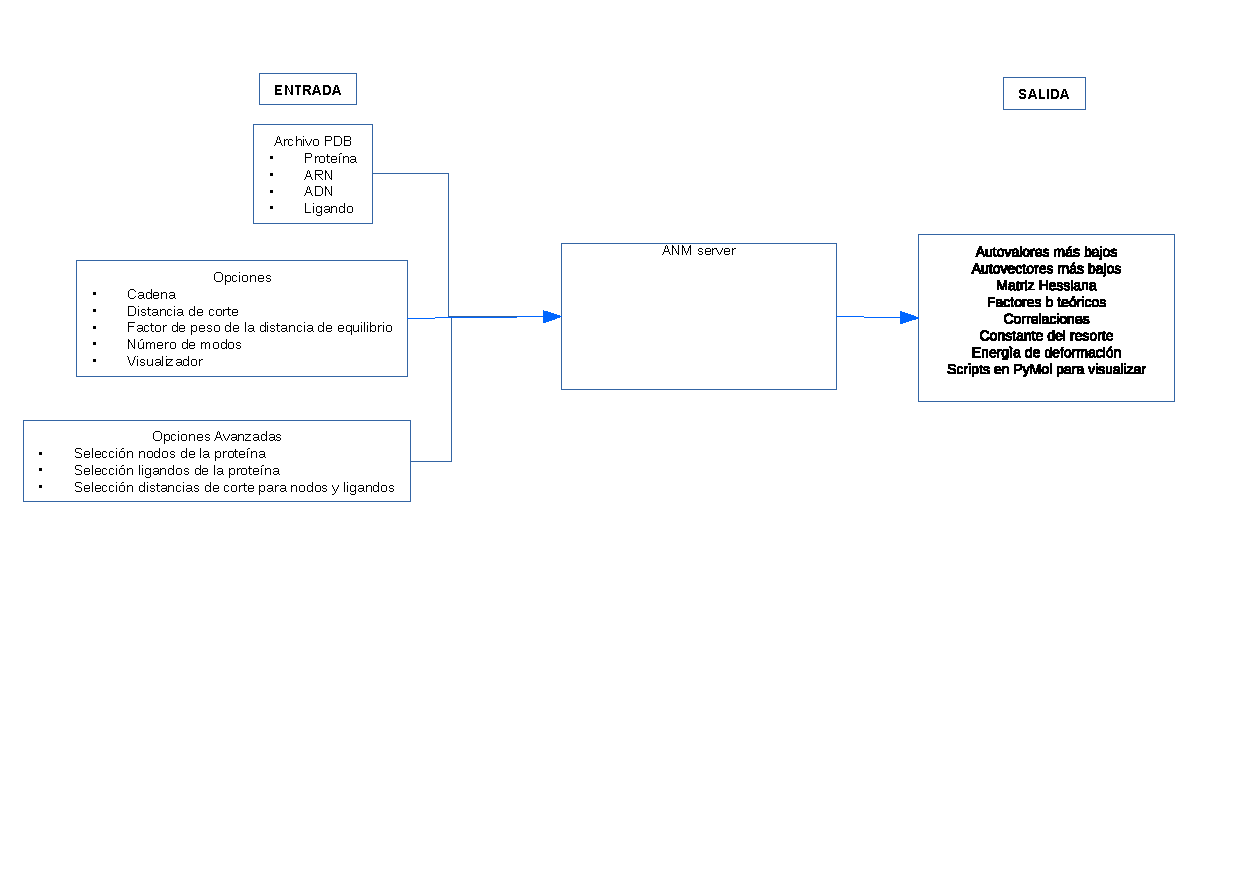
\includegraphics[scale=0.6]{./Kap4/flujo.pdf} 
\caption{Esquema de entrada y salida del servidor ANM}\label{fig:flujo}
\end{figure}

\section{NMA previo de vSGLT}
\subsection{Metodolog\'{i}a}
Mediante el servidor ANM, se ha realizado un estudio previo del simportador vSGLT   \cite{Cabrera2017} , en el cual se utiliza el archivo de entrada 3dh4.pdb \cite{Faham2008} encontrado en la base de datos del PDB como tetr\'{a}mero. En este archivo pdb no se determinan los residuos de la primera h\'{e}lice en cada subunidad. Aunque aparecen las posiciones de los residuos, el ANM server los ignora, haciendo el c\'{a}lculo \'{u}nicamente a partir del residuo 47.\\

Una vez ingresado el archivo pdb se selecciona el modelo de la estructura. Inicialmente se toman s\'{o}lamente los carbonos $\alpha$ del co-transportador, se seleccionan las distancias de corte $R_c$ entre $7\AA$ y $14\AA$. Adem\'{a}s, el factor de peso aplicado a las distancias de corte es $s=0$, es decir, las distancias de corte en el hessiano \eqref{eq:hes} son fijas \cite{Zimmermann2011}. Luego se calculan los modos normales $(\lambda_k,a_k)$ (autovalores, autovectores) y los factores b mediante la parte del c\'{o}digo escrita en Fortran. Se hace otro NMA agregando los \'{a}tomos de la galactosa (sin hidr\'{o}genos), agregando el sodio y luego agregando tanto el ion como el sustrato.\\
\subsection{Resultados}
En la figuras \ref{fig:ANM_pre1}, \ref{fig:ANM_pre2}, \ref{fig:ANM_pre3} y \ref{fig:ANM_pre4} se muestran los factores b por cada n\'{u}mero de residuo (entre 47 y 545) y para cada distancia de corte $R_c$, entre $8\AA$ y $14\AA$ de la cadena A. Ha de notarse que para distancias de corte menores o iguales a $7\AA$,no se encontraron todos  los autovalores, ni autovectores, ni factores b, ya que no todos los autovalores convergen \cite{Zimmermann2011}.\\

\begin{figure}[ht]
 \centering
 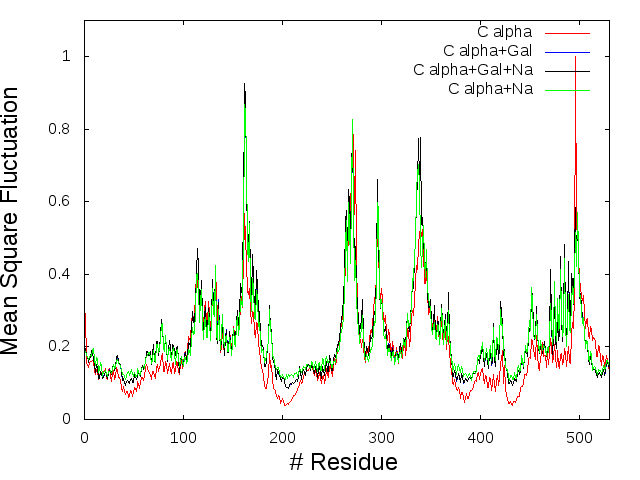
\includegraphics[scale=0.35]{./Kap4/ANM/ANM_server/grafica_8_A_n.png}
  \put(-28,-4){(a) $R_c=8\AA$}
   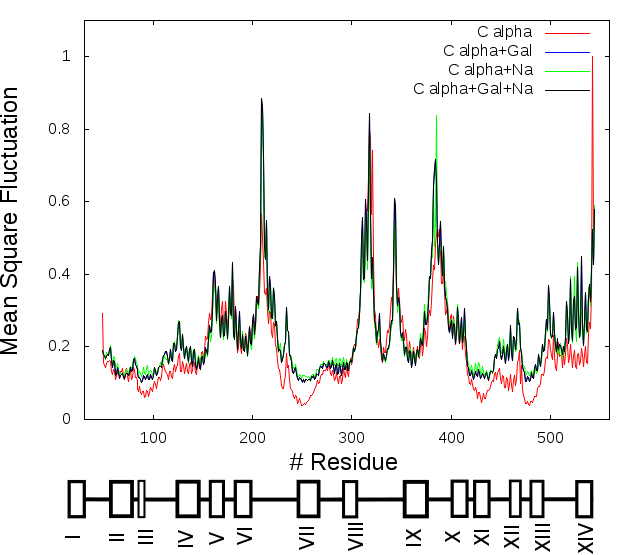
\includegraphics[scale=0.35]{./Kap4/ANM/ANM_server/grafica_9_A_n.png}
  \put(-28,-4){(b) $R_c=9\AA$}
\caption{Fluctuaciones ms normalizadas en funci\'{o}n del n\'{u}mero de residuo para $ R_c=8\AA$ y $R_c= 9\AA$ usando  los primeros 100 modos. Los diferentes colores indican si la simulaci\'{o}n fue realizada sin el ion, el sustrato, con alguno de ellos o ambos.}\label{fig:ANM_pre1}
\end{figure}

Para distancias de corte entre $8\AA$ y $9\AA$, se observa en las gr\'{a}ficas \ref{fig:ANM_pre1} (a) y (b) que la prote\'{i}na  es menos flexible cuando est\'{a} sin unirse a los sustratos (color rojo) desde el segmento TM2 hasta el final del segmento TM14. La excepci\'{o}n es el pico presente en el residuo W543 (Cuyo factor b est\'{a} en tabla \ref{tab:flu2} del anexo \ref{AnexoB}) que presenta mucha m\'{a}s flexibilidad. Esto se debe a que el segmento TM14 est\'{a} lejos tanto del sitio activo de la prote\'{i}na como de la segunda subunidad como se observa en la figura \ref{fig:complejo} donde TM14 es la $\alpha$ h\'{e}lice de color rojo.\\

Los picos correspondientes a los residuos S209 y F210 tambi\'{e}n muestran cambios significativos de la fluctuaciones ms antes y despu\'{e}s de unirse alguno de los sustratos. Estos picos corresponden al comienzo al lazo $\omega$ comprendido entre las segmentos TM6 y TM7.\\

El co-transportador es m\'{a}s flexible cuando al menos uno de los sustratos se encuentra unido al simportador. Pero los movimientos globales de simportador no difieren significativamente cuando el ion, el soluto o ambos est\'{a}n unidos. Esto podr\'{i}a sugerir que el \ce{Na^{+}} y la galactosa no son de alta cooperaci\'{o}n.\\

Para comprobar esta afirmaci\'{o}n se hace una mirada detallada a las regiones alrededor de los residuos Ile253, Glu88, Phe479, Ile438 y la regi\'{o}n con los residuos Glu384,Tyr385 y Ile386.\\
\begin{figure}[h]
 \centering
    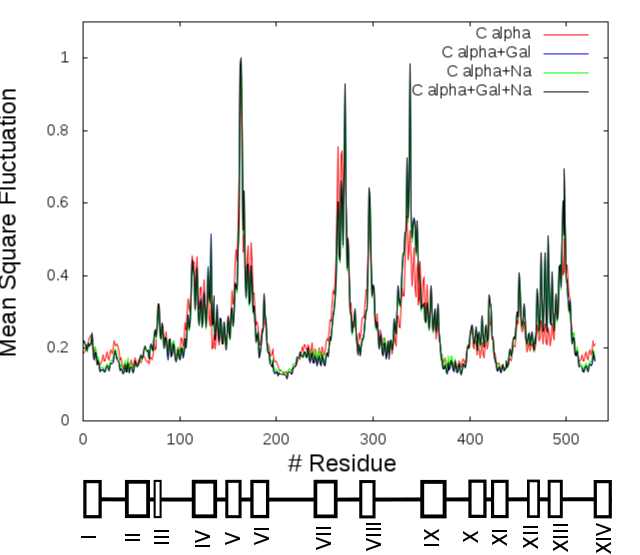
\includegraphics[scale=0.35]{./Kap4/ANM/ANM_server/grafica_10_A_n.png}
   \put(-28,-4){(a)$R_c=10\AA$}
\caption{Fluctuaciones ms normalizadas en funci\'{o}n del n\'{u}mero de residuo para $ R_c=10\AA$ usando  los primeros 100 modos. Los diferentes colores indican si la simulaci\'{o}n fue realizada sin el ion, el sustrato, con alguno de ellos o ambos.}\label{fig:ANM_pre2}
\end{figure}
\begin{figure}[h]
 \centering
     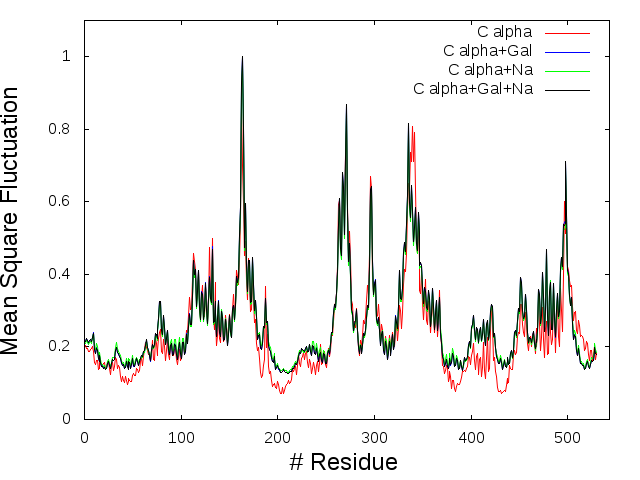
\includegraphics[scale=0.35]{./Kap4/ANM/ANM_server/grafica_11_A_n.png}
    \put(-28,-4){(a)$R_c=11\AA$}
      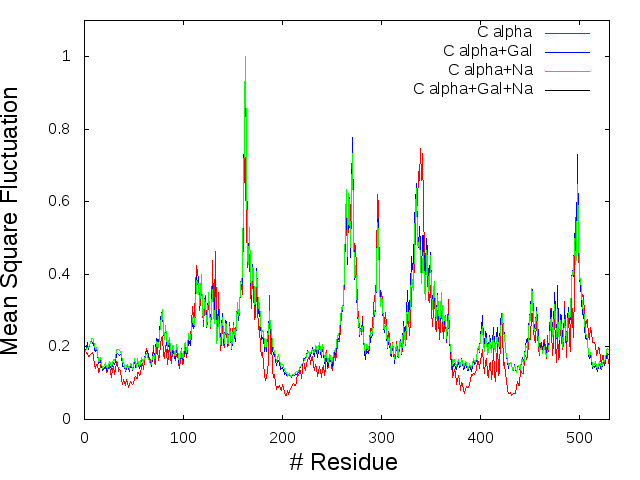
\includegraphics[scale=0.35]{./Kap4/ANM/ANM_server/grafica_12_A_n.png}
     \put(-28,-4){(a)$R_c=12\AA$}
\caption{Fluctuaciones ms normalizadas en funci\'{o}n del n\'{u}mero de residuo para $ R_c=11\AA$ y $R_c= 12\AA$ usando  los primeros 100 modos. Los diferentes colores indican si la simulaci\'{o}n fue realizada sin el ion, el sustrato, con alguno de ellos o ambos.}\label{fig:ANM_pre3}
\end{figure}
\begin{figure}[h]
 \centering
       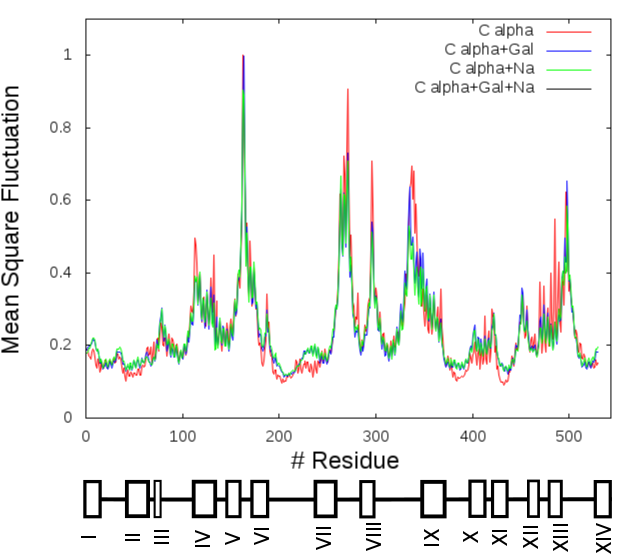
\includegraphics[scale=0.35]{./Kap4/ANM/ANM_server/grafica_13_A_n.png}
     \put(-28,-4){(a)$R_c=13\AA$}
       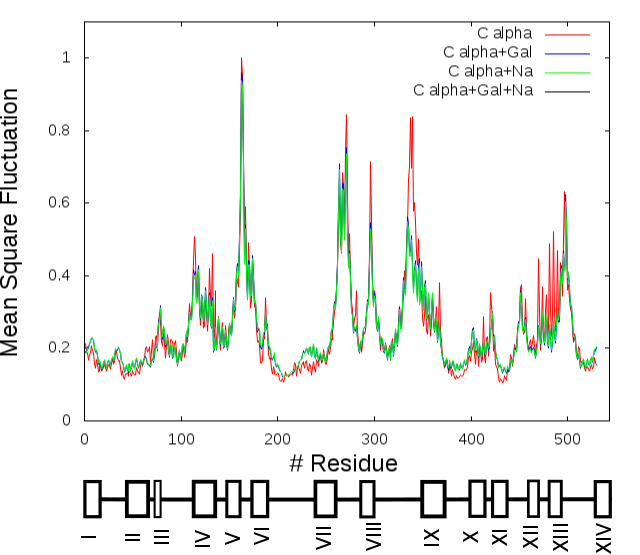
\includegraphics[scale=0.35]{./Kap4/ANM/ANM_server/grafica_14_A_n.png}
\put(-28,-4){(a)$R_c=14\AA$}

\caption{Fluctuaciones ms normalizadas en funci\'{o}n del n\'{u}mero de residuo para $ R_c=13\AA$ y $R_c= 14\AA$ usando  los primeros 100 modos. Los diferentes colores indican si la simulaci\'{o}n fue realizada sin el ion, el sustrato, con alguno de ellos o ambos.}\label{fig:ANM_pre4}
\end{figure}
 

Para $Rc = 8\AA$ y $Rc = 9\AA$, los movimientos en TM7 (entre los residuos 192-214), TM11 (residuos 372-393), TM12 (residuos 423-493) cuando Na + y Gal est\'{a}n unidos son ligeramente menos r\'{i}gidos ($<5\%$ ) Que los movimientos de vSGLT con un sitio ocupado. TM7 regi\'{o}n es importante porque Y263 act\'{u}an como una puerta y Gal interact\'{u}a con Y263 y N260.\\
For $Rc=8\AA$,  $9\AA$ and $11\AA$, the motions in TM6 (residues 161-167), especially T162 and TM13 in residue F496  when Na+ and Gal are bound are more rigid than  motions of vSGLT alone.\\
Para $Rc = 8\AA$, $9\AA$ y $11\AA$, hay otros residuos involucrados en cambios de movimientos, estos son en segmentos mencionados anteriormente.\\

\section{ANM de vSGLT con la Estructura Completa}
\subsection{Preparaci\'{o}n del PDB}
Ya que en el mutante de vSGLT en la posici\'{o}n K294A, llamado 2XQ2 aparece resuelta la estructura cristalina del TM1 perteneciente a la cadena A, se usa el programa PyMol, y como archivos de entrada los pdbs 3DH4 y el de su mutante 2XQ2, para crear un archivo que sea cercano a la estructura real objeto de estudio, esto es, al cotransportador vSGLT. Se a\~{n}ade a 3DH4 la h\'{e}lice 1 resuelta, tal como aparece en la figura 
\begin{figure}[H]
 \centering
 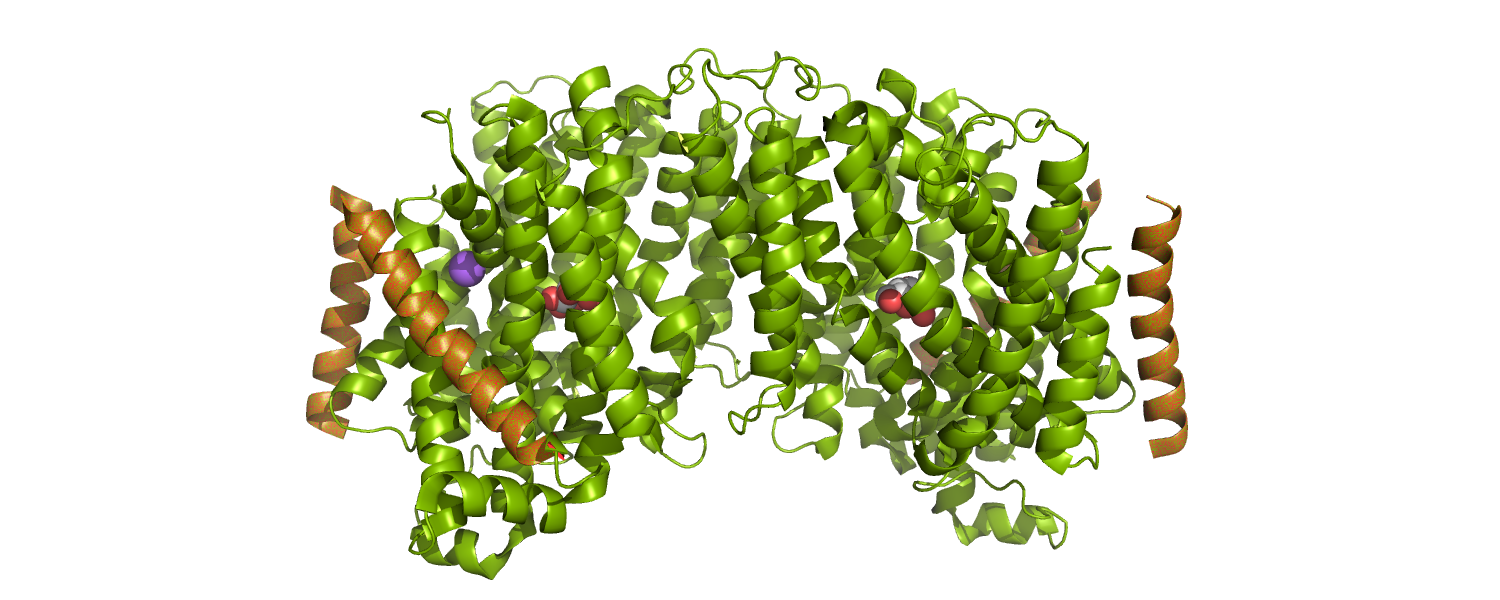
\includegraphics[scale=0.3]{Kap4/vSGLT_n.png}
 % vSGLT_n.png: 0x0 pixel, 300dpi, 0.00x0.00 cm, bb=
 \caption{Estructura del cotransportador vSGLT en su conformaci\'{o}n ocluida junto con las h\'{e}lices 1 y 15 a\~{n}adidas mediante PyMol.}
 \label{fig:vSGLT_in_2}
\end{figure}

\subsection{Resultados}
En la figuras \ref{fig:ANM_pos1}, \ref{fig:ANM_pos2}, \ref{fig:ANM_pos3} y \ref{fig:ANM_pos4} se muestran los factores b por cada n\'{u}mero de residuo (entre 47 y 545) y para cada distancia de corte $R_c$, entre $8\AA$ y $20\AA$ de la cadena A. Ha de notarse que al igual que el ANM previo, para distancias de corte menores o iguales a $7\AA$,no se encontraron todos  los autovalores, ni autovectores, ni factores b, ya que no todos los autovalores convergen \cite{Zimmermann2011}.\\
\begin{figure}[h]
 \centering
 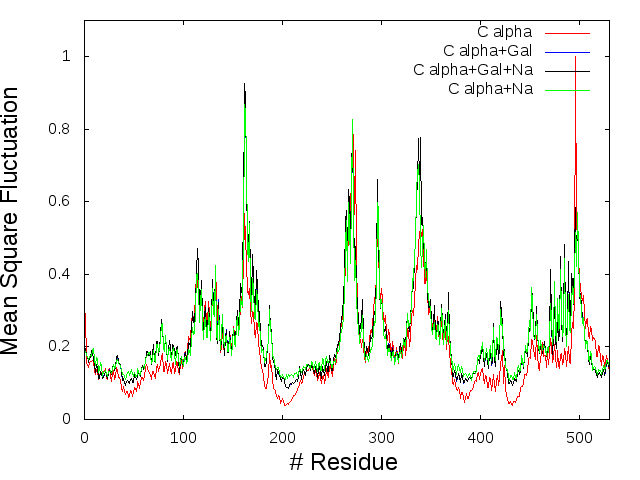
\includegraphics[scale=0.3]{./Kap4/ANM/ANM_server/grafica_8_A_n.png}
  \put(-28,-4){(a) $R_c=8\AA$}
   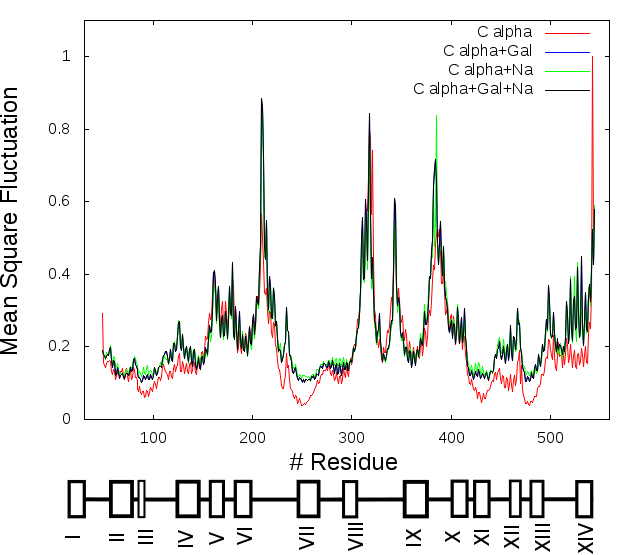
\includegraphics[scale=0.3]{./Kap4/ANM/ANM_server/grafica_9_A_n.png}
  \put(-28,-4){(b) $R_c=9\AA$}
\caption{Fluctuaciones ms normalizadas en funci\'{o}n del n\'{u}mero de residuo para $ R_c=8\AA$ y $R_c= 9\AA$ usando  los primeros 100 modos. Los diferentes colores indican si la simulaci\'{o}n fue realizada sin el ion, el sustrato, con alguno de ellos o ambos.}\label{fig:ANM_pos1}
\end{figure}

\begin{figure}[h]
 \centering
    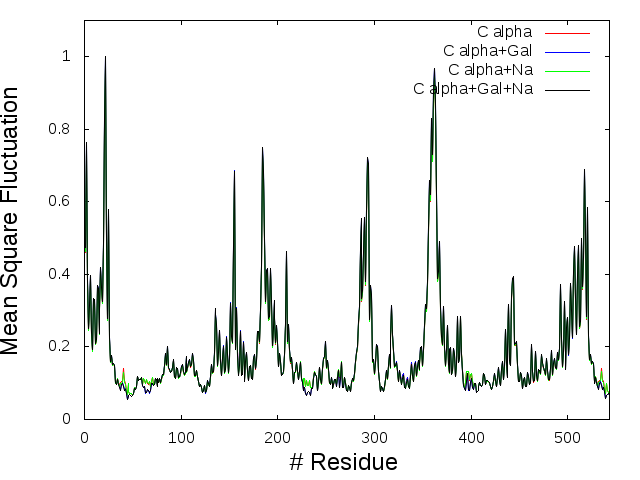
\includegraphics[scale=0.35]{./Kap4/ANM/ANM_s_nuevo/grafica_10_A_n.png}
   \put(-28,-4){(a)$R_c=10\AA$}
     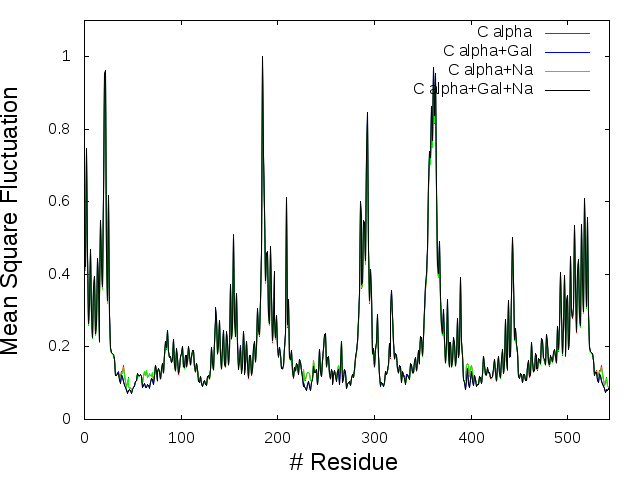
\includegraphics[scale=0.35]{./Kap4/ANM/ANM_s_nuevo/grafica_11_A_n.png}
    \put(-28,-4){(b)$R_c=11\AA$}
     \vspace{1mm}
      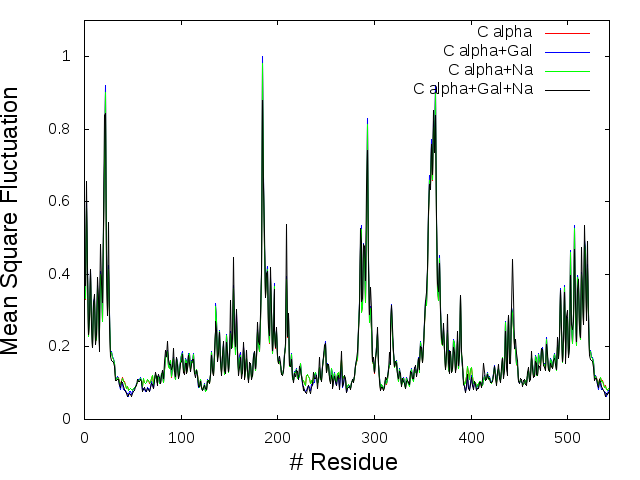
\includegraphics[scale=0.35]{./Kap4/ANM/ANM_s_nuevo/grafica_12_A_n.png}
     \put(-28,-4){(c)$R_c=12\AA$}
       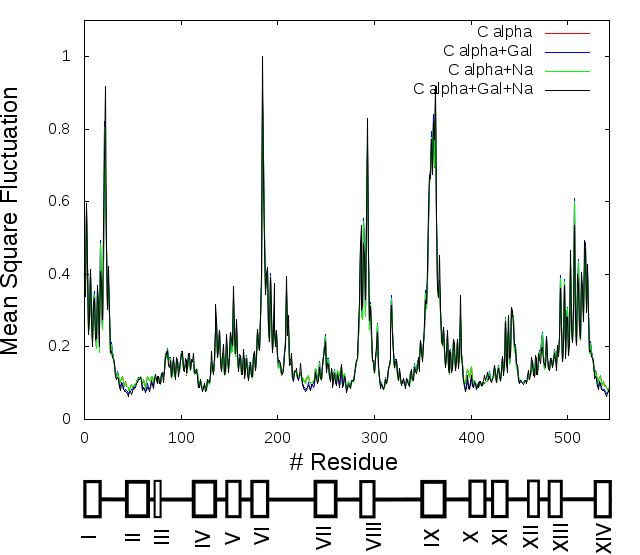
\includegraphics[scale=0.35]{./Kap4/ANM/ANM_s_nuevo/grafica_13_A_n.png}
     \put(-28,-4){(d)$R_c=13\AA$}
\caption{Fluctuaciones ms normalizadas en funci\'{o}n del n\'{u}mero de residuo para $ R_c=10\AA$ y $R_c= 13\AA$ usando  los primeros 100 modos. Los diferentes colores indican si la simulaci\'{o}n fue realizada sin el ion, el sustrato, con alguno de ellos o ambos.}\label{fig:ANM_pos2}
\end{figure}
\begin{figure}[h]
 \centering
    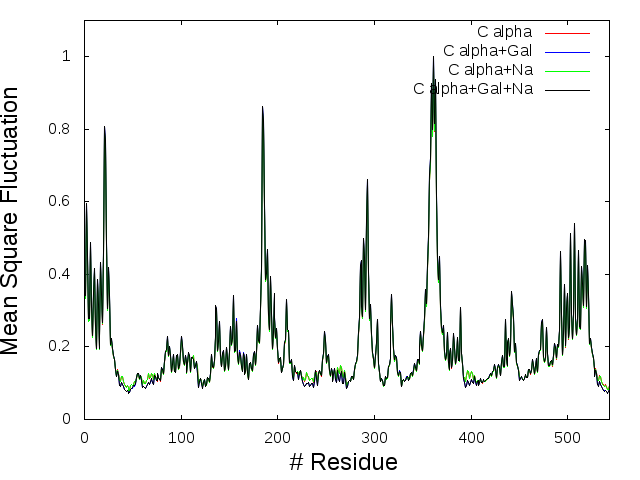
\includegraphics[scale=0.35]{./Kap4/ANM/ANM_s_nuevo/grafica_14_A_n.png}
   \put(-28,-4){(a)$R_c=14\AA$}
     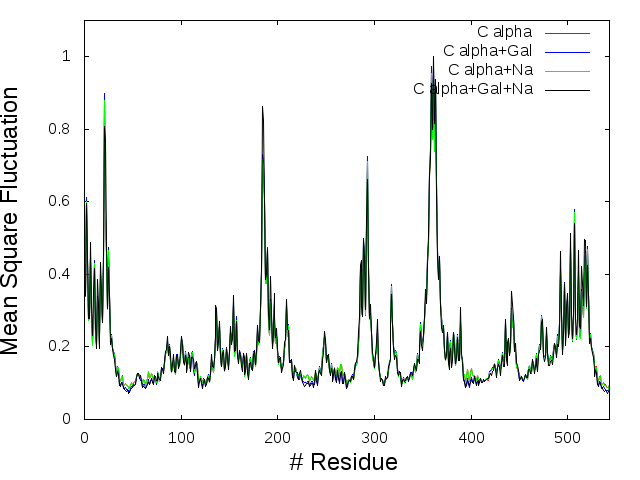
\includegraphics[scale=0.35]{./Kap4/ANM/ANM_s_nuevo/grafica_15_A_n.png}
    \put(-28,-4){(b)$R_c=15\AA$}
    \vspace{1mm}
      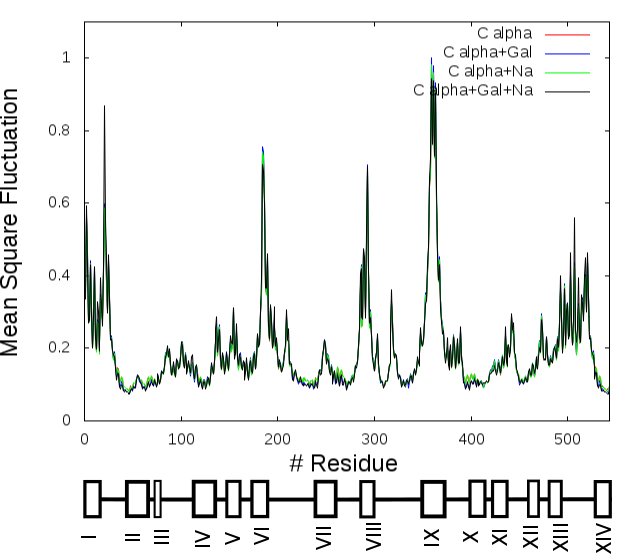
\includegraphics[scale=0.35]{./Kap4/ANM/ANM_s_nuevo/grafica_16_A_n.png}
     \put(-28,-4){(c)$R_c=16\AA$}
       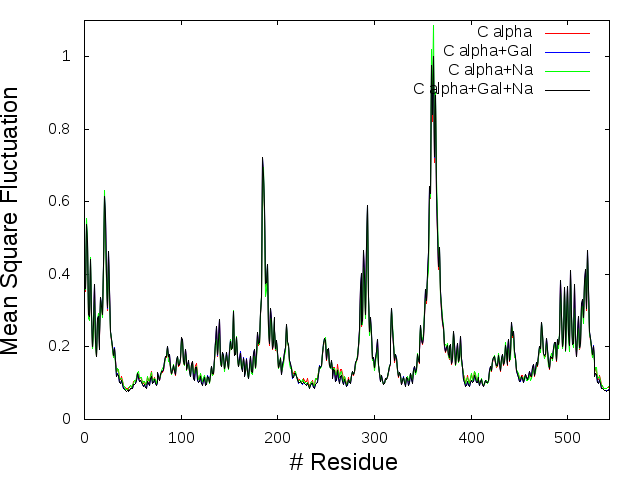
\includegraphics[scale=0.35]{./Kap4/ANM/ANM_s_nuevo/grafica_17_A_n.png}
     \put(-28,-4){(d)$R_c=17\AA$}
\caption{Fluctuaciones ms normalizadas en funci\'{o}n del n\'{u}mero de residuo para $ R_c=14\AA$ y $R_c= 17\AA$ usando  los primeros 100 modos. Los diferentes colores indican si la simulaci\'{o}n fue realizada sin el ion, el sustrato, con alguno de ellos o ambos.}\label{fig:ANM_pos3}
\end{figure}
\begin{figure}[h]
 \centering
    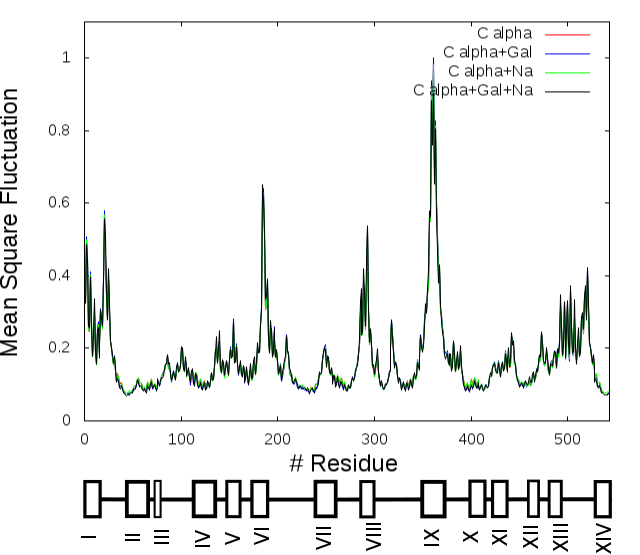
\includegraphics[scale=0.35]{./Kap4/ANM/ANM_s_nuevo/grafica_18_A_n.png}
   \put(-28,-4){(a)$R_c=18\AA$}
     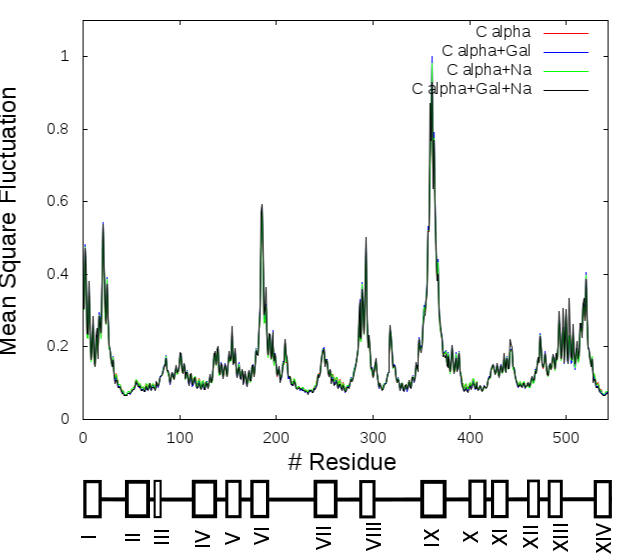
\includegraphics[scale=0.35]{./Kap4/ANM/ANM_s_nuevo/grafica_19_A_n.png}
    \put(-28,-4){(b)$R_c=19\AA$}
     \vspace{1mm}
      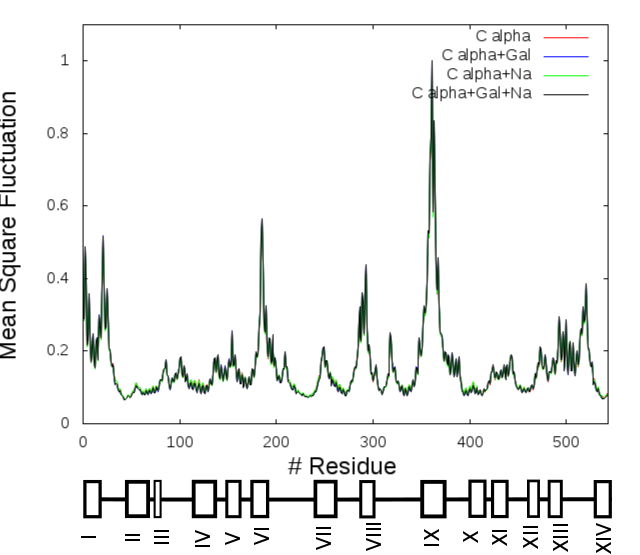
\includegraphics[scale=0.35]{./Kap4/ANM/ANM_s_nuevo/grafica_20_A_n.png}
     \put(-28,-4){(c)$R_c=20\AA$}
\caption{Fluctuaciones ms normalizadas en funci\'{o}n del n\'{u}mero de residuo para $ R_c=18\AA$ y $R_c=20\AA$ usando  los primeros 100 modos. Los diferentes colores indican si la simulaci\'{o}n fue realizada sin el ion, el sustrato, con alguno de ellos o ambos.}\label{fig:ANM_pos4}
\end{figure}